\chapter{Implementación}
\label{ch:chap04}

\section{OpenGL}
\label{sec:opengl-impl}

\subsection{Cálculo de factores de forma de la componente difusa}

El \textit{pipeline} de cáculo de factores de forma utilizando OpenGL se compone de tres etapas principales.

Etapa 1:

En primera instancia, se configurarán los \textit{buffers} de memoria necesarios para representar el hemi-cubo que se dibujará.

Para ello, se crea un \textit{Frame Buffer Object} en la GPU que estará compuesto de 5 texturas, cada una de ellas correspondiente a una de las caras a dibujar. Cabe destacar, que estas texturas se compondrán de dos imágenes, una de ellas contiene enteros sin signo que serán utilizados para representar un \verb|id| de cara parche de la escena y la restante contiene los valores de profundidad necesarios para el algoritmo del Z-Buffer.

Etapa 2:

En la segunda etapa se procede al renderizado y procesado de cada uno de los hemi-cubos. Para ello, se procede como en \ref{alg:hemicube}.

\begin{minipage}{\linewidth}
\label{alg:hemicube}
\begin{lstlisting}[language=C]
global formFactorMatrix;

void processHemicube(face, hemicube){
	row = [0,...,0]
	for (pixel in hemicube) {
		factor = getHemicubeCorrection(pixel);
		seenFace = getFaceId(pixel);
		if (isValid(seenFace)){
			row[seenFace] += factor
		}
	}
	formFactorMatrix[face] = row;
}

computeFormFactors() {
	bindHemicube()
	for (face in scene){
		alignCamera(face);
		clearBuffers();
		render(scene);
		hemicube = getHemicube();
		startThread(processHemicube, face, hemicube)
	}
}

\end{lstlisting}
\end{minipage}

El proceso de renderizado del hemicubo es realizado completamente en la GPU, sin embargo tiene características particulares que diferencial el proceso de otras implementaciones del algoritmo. 

Con el objetivo de tener el mejor rendimiento posible, se hace uso de los \textit{geometry shaders} para realizar una única llamada de dibujado por objeto. Además, como puede apreciarse en la figura \ref{img:statechangescost}, el método posibilita el cambio de \textit{render target} una única vez, al comienzo del dibujado como se ilustra en \ref{alg:hemicube} solo se realiza una única llamada de \textit{binding} del hemi-cubo .

\vspace{5mm}
\begin{minipage}[h]{\linewidth}
	\centering
	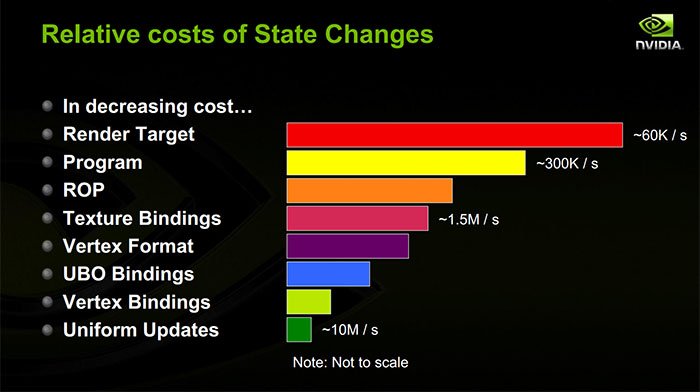
\includegraphics[width=\linewidth]{assets/statecosts}
	\captionof{figure}{Costo de cambios de estado en OpenGL. Fuente: Nvidia}
	\label{img:statechangescost}
\end{minipage}

El proceso consiste entonces en el dibujado de cinco texturas en simultáneo. 

\begin{enumerate}
	\item El \textit{vertex shader} es simplemente \textit{passthough} lo que signfica que conecta las entradas proveídas por la CPU con su salida.
	\item El \textit{geometry shader} genera cinco primitivas donde cada una estará en las coordenadas correspondientes a los frustums de las caras del hemicubo además de añadir un plano adicional de corte del dibujo necesario debido a la imposibilidad de que las caras laterales posean una resolución menor a la cara superior.
	\item El \textit{fragment shader} corregirá y escribirá el identificador de la cara detectada en la textura que le corresponda.
\end{enumerate}

\subsection{Cálculo de factores de forma de la componente especular}

\subsubsection{OpenGL}

\subsubsection{Embree}

\section{Embree}
\label{sec:embree-impl}

\subsection{Cálculo de factores de forma de la componente difusa}

\subsection{Cálculo de factores de forma de la componente especular}


\section {Interfaz de usuario}
